% --- SECTION 4: EMPIRICAL RESULTS ---
\section{Empirical Results}

\subsection{Implementation Details}

The Monte Carlo reinforcement learning agent was implemented in \textbf{Python 3.10} using the following key libraries:

\begin{itemize}
    \item \texttt{PyTorch} for neural network policy and value function implementation
    \item \texttt{NumPy} and \texttt{Pandas} for data manipulation and feature engineering
    \item \texttt{gym-trading-env} as the trading environment
    \item \texttt{Matplotlib} and \texttt{Seaborn} for visualization of learning curves and results
\end{itemize}

\subsubsection{Environment Setup}
Gym Trading Env \citep{gymtradingenv} is a Gymnasium environment for simulating stocks and training Reinforcement Learning (RL) trading agents. It was designed to be fast and customizable for easy RL trading algorithms implementation. The trading environment was configured to simulate daily trading on the DAX index using the preprocessed dataset described in Section 3.

To ensure robustness, the agents were trained using \textbf{10 different random seeds}. This allows for an assessment of variability in learning outcomes and provides reliable statistical estimates of agent performance. 

\subsubsection{Neural Network Architecture and Hyperparameters}
The policy network consists of two fully connected hidden layers with 128 units each, using ReLU activation functions. The network outputs action probabilities via a softmax layer. For the baseline variant, a separate value network with identical architecture (except for a single output unit) estimates state values. Both networks are optimized using the \textbf{Adam} optimizer with a learning rate of \textbf{1e-3} and a discount factor $\gamma = 0.99$. Gradient clipping with a maximum norm of 1.0 is applied to stabilize training, and returns are normalized before computing policy gradients to reduce variance.

\begin{figure}[htbp]
    \centering
    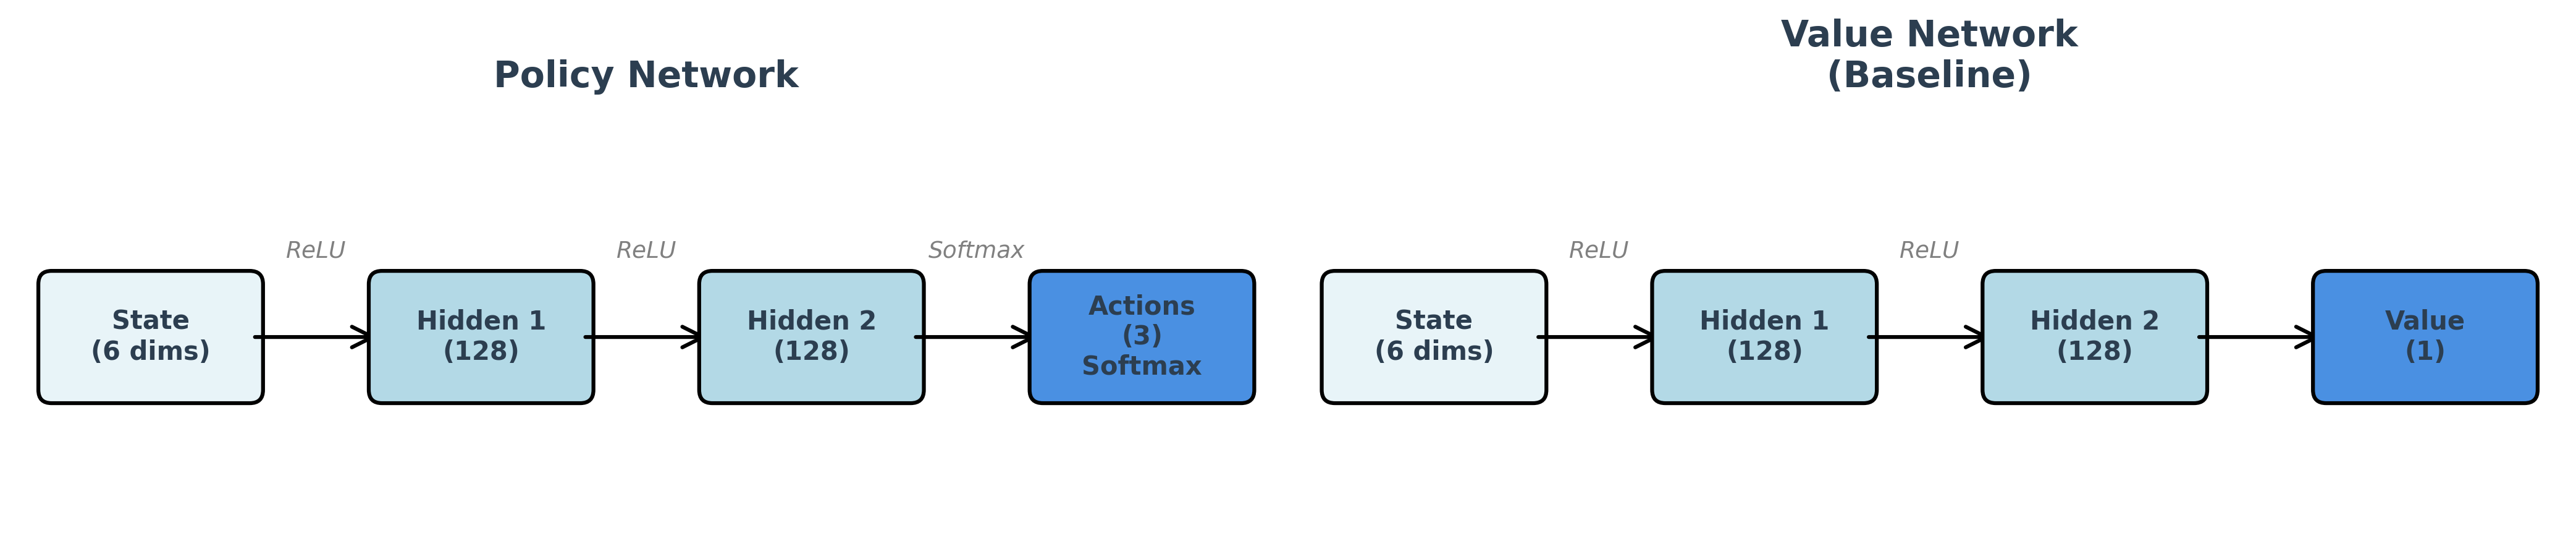
\includegraphics[width=0.8\textwidth]{../report/figures/model_architecture.png}
    \caption{Overview of the neural network architecture for the REINFORCE agent. The policy network (left) maps states to action probabilities, while the value network (right, used in the baseline variant) estimates state values.}
    \label{fig:model_architecture}
\end{figure}


\subsection{Empirical Results}

This section presents the empirical findings of the Monte Carlo policy gradient agents trained on historical DAX data. 
The methods compared are REINFORCE without baseline, REINFORCE with a learned value-function baseline, 
and a random trading strategy serving as a lower-bound benchmark.

\subsubsection{Learning Dynamics and Convergence}

\begin{figure}[htbp]
    \centering
    \begin{subfigure}[t]{0.48\textwidth}
        \centering
        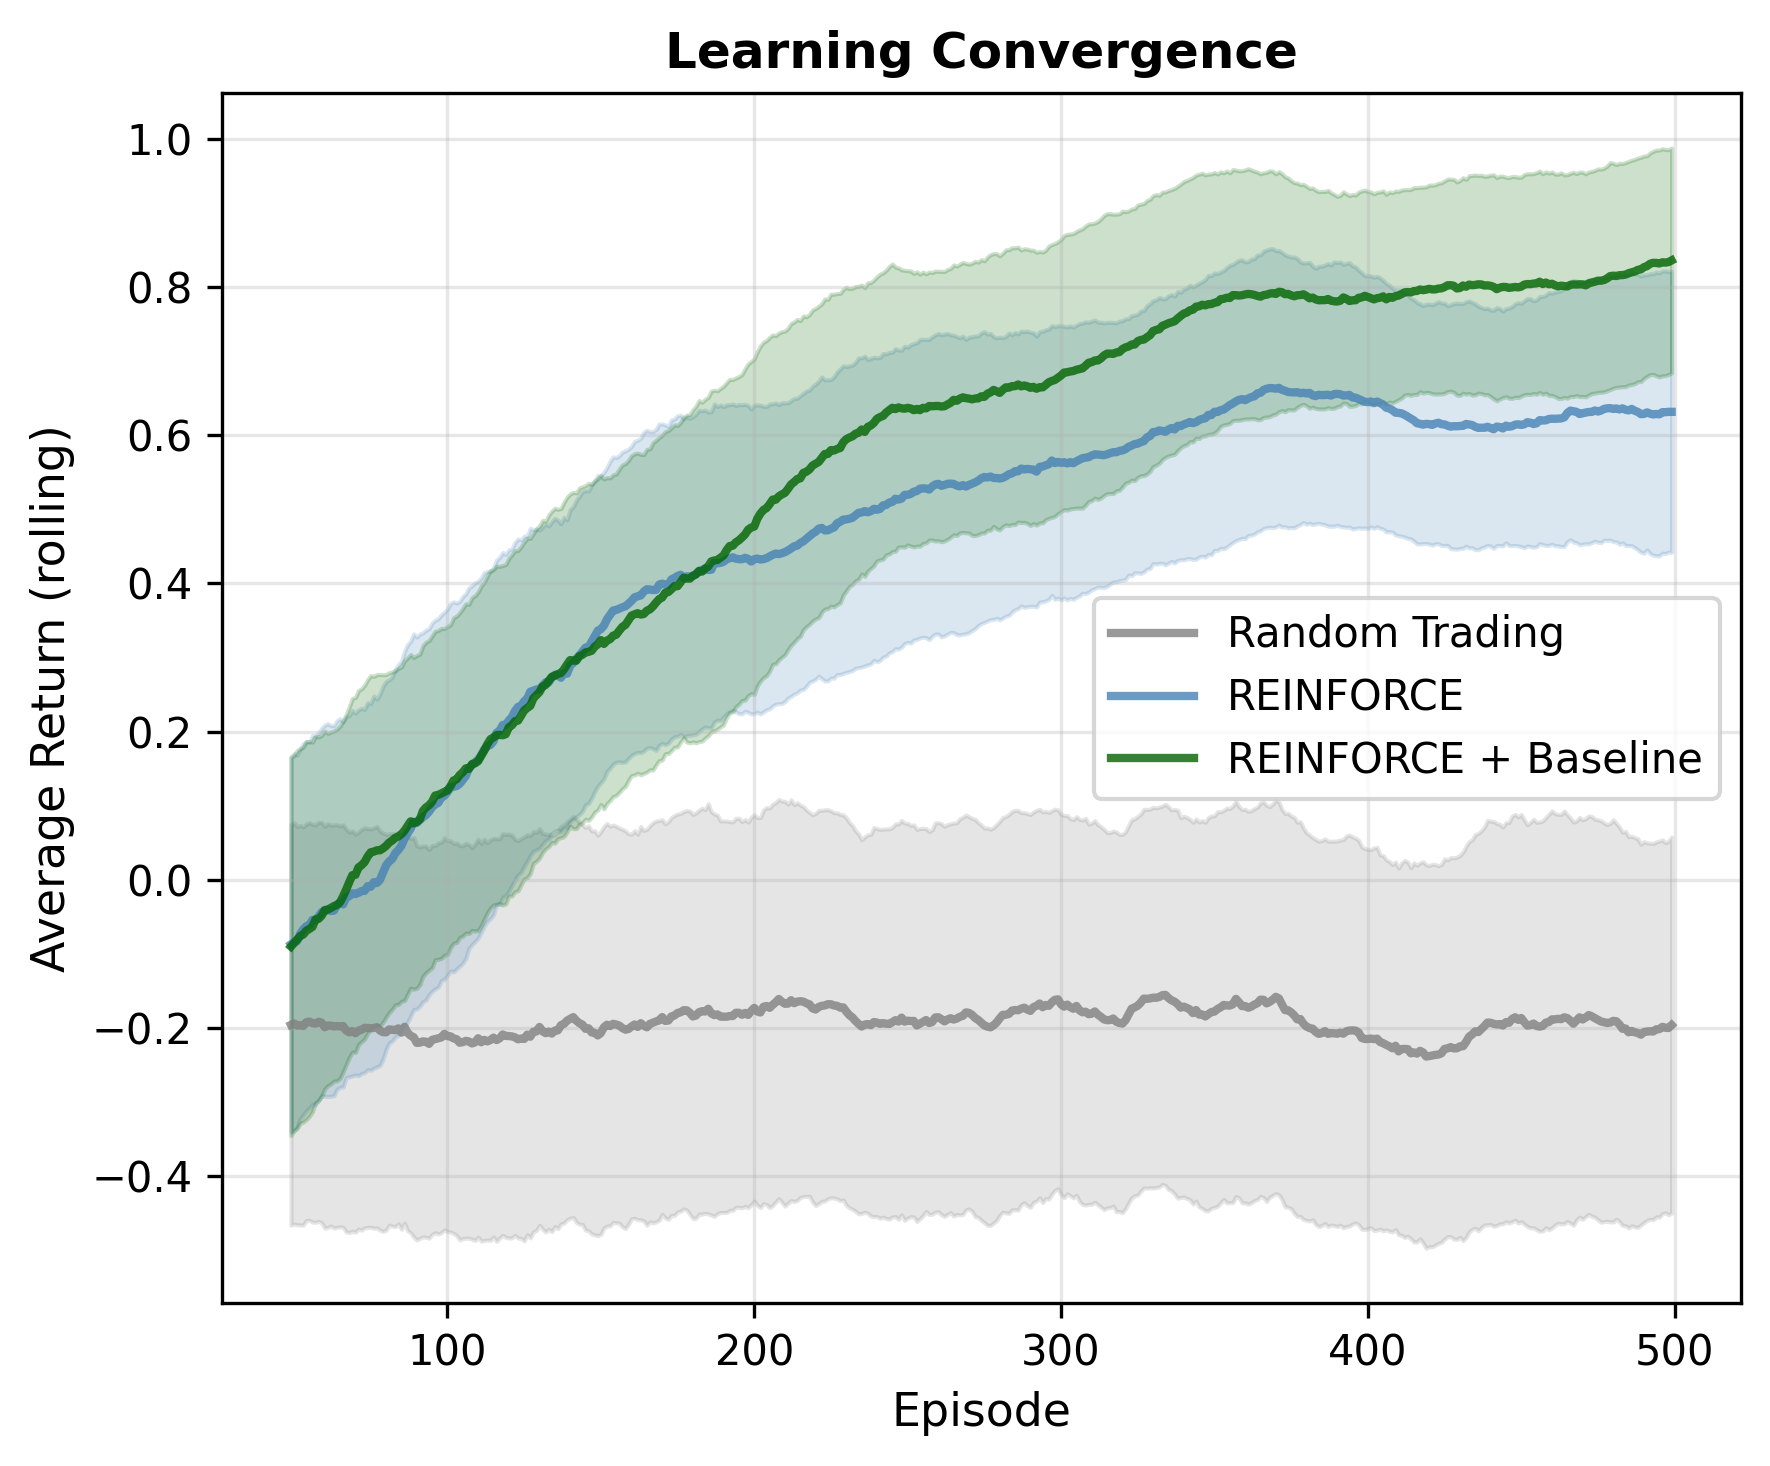
\includegraphics[width=\textwidth]{../report/figures/convergence_convergence.png}
        \caption{Learning convergence: Rolling average episode return across 10 random seeds.}
        \label{fig:learning_convergence}
    \end{subfigure}
    \hfill
    \begin{subfigure}[t]{0.48\textwidth}
        \centering
        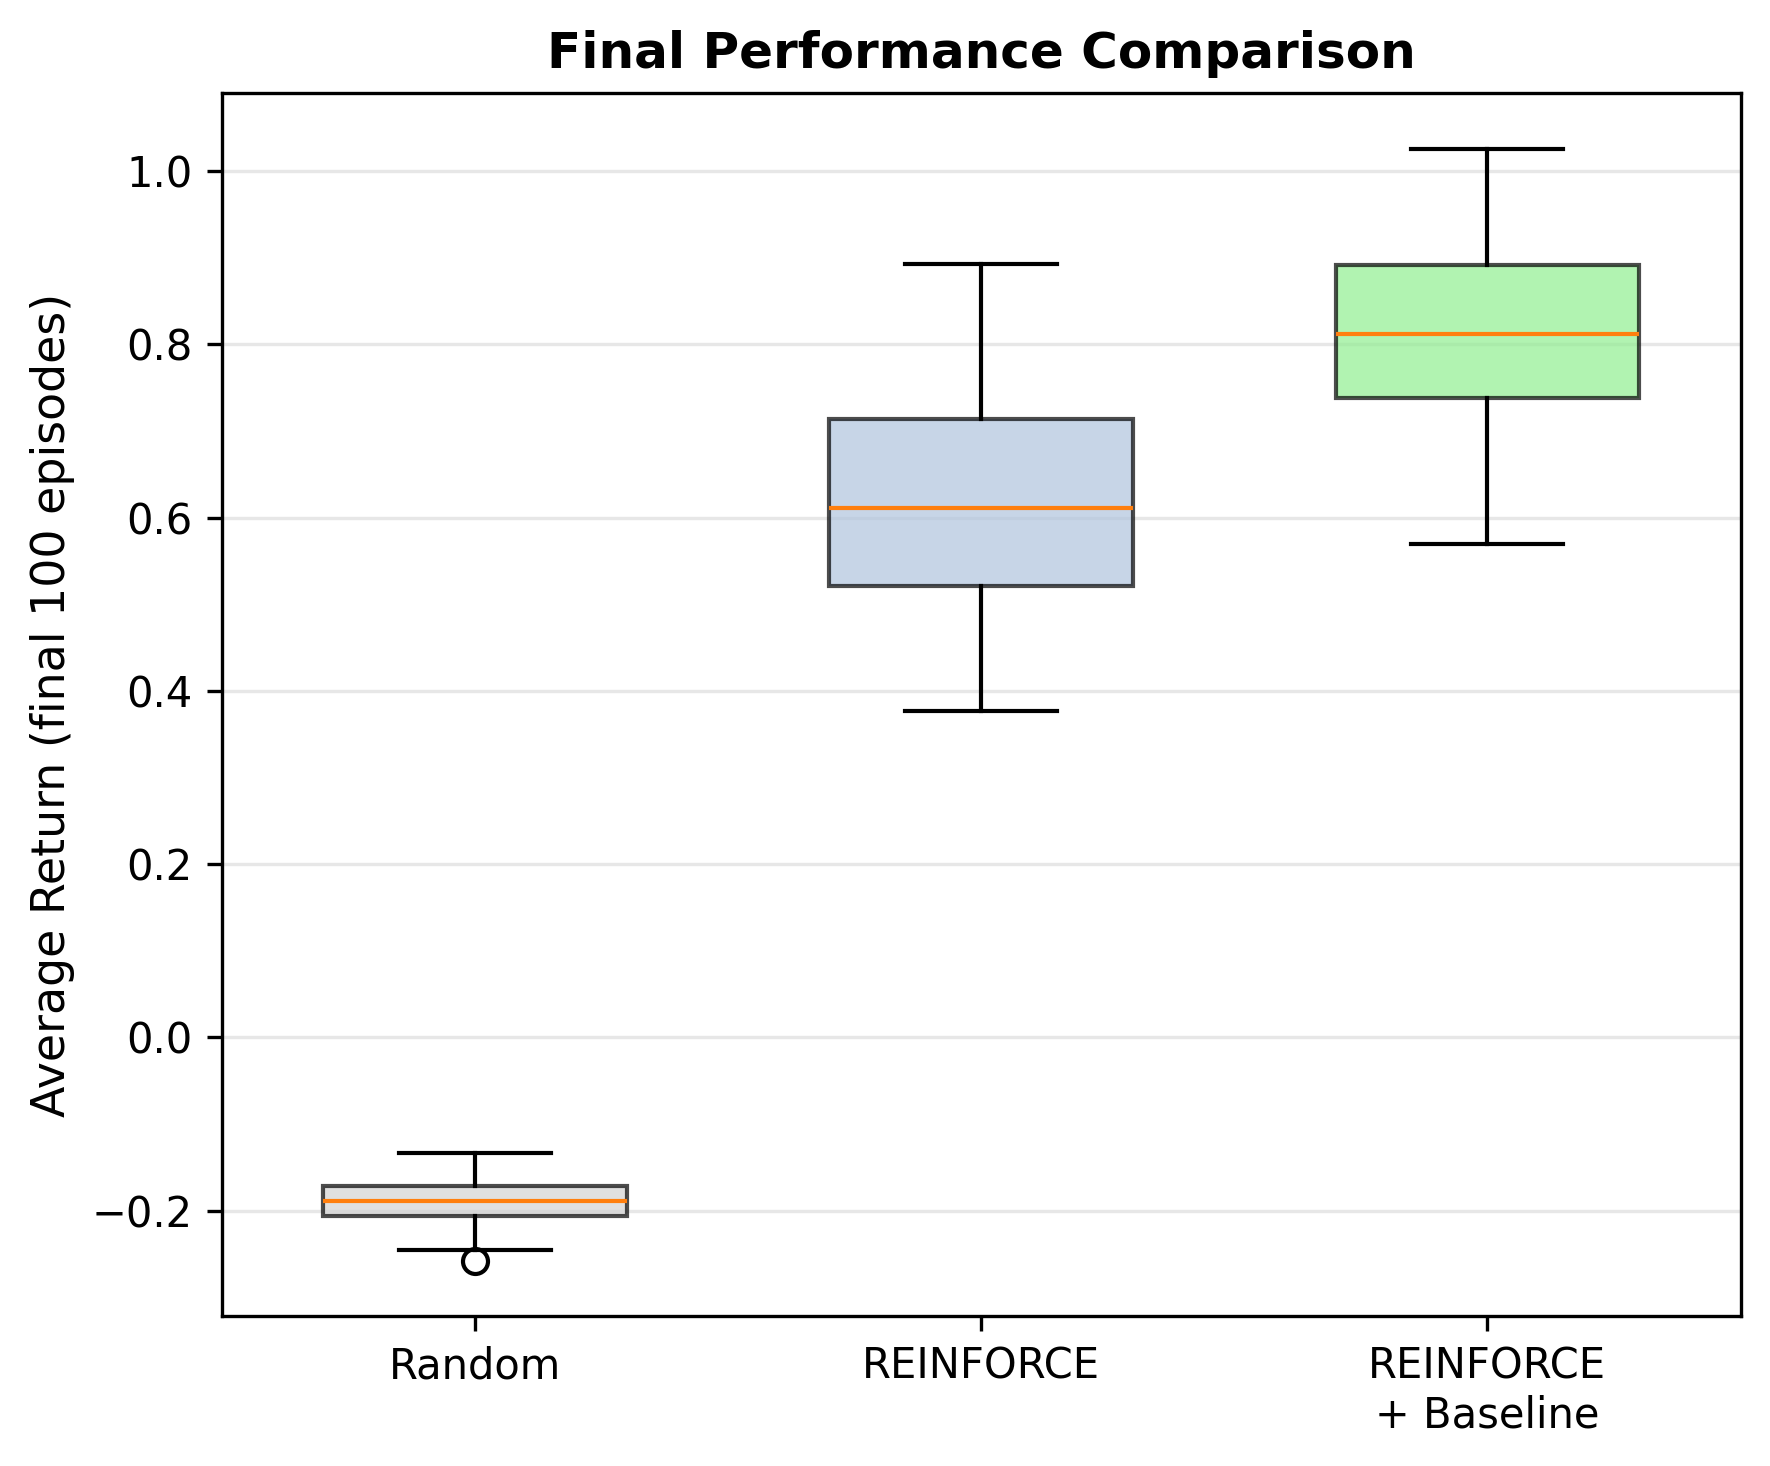
\includegraphics[width=\textwidth]{../report/figures/convergence_final_performance.png}
        \caption{Boxplot comparing average returns in the final 100 episodes.}
        \label{fig:performance_comparison}
    \end{subfigure}
\end{figure}


Figure~\ref{fig:learning_convergence} shows the rolling average return per episode. 
The REINFORCE agent with baseline converges faster and exhibits smoother learning curves compared to 
the standard REINFORCE agent. This supports the theoretical expectation that incorporating a value-function baseline 
reduces gradient variance and stabilizes learning.

Figure~\ref{fig:performance_comparison} presents a boxplot of the average return over the final 100 episodes. 
The baseline variant achieves higher median returns and a narrower interquartile range, 
indicating improved performance and reduced variability across seeds. 
The random policy displays the dispersion centered around -0.2, confirming its role as a benchmark 
without learning capability.

\subsubsection{Return Distribution and Risk Analysis}

\begin{figure}[htbp]
    \centering
    \begin{subfigure}[t]{0.48\textwidth}
        \centering
        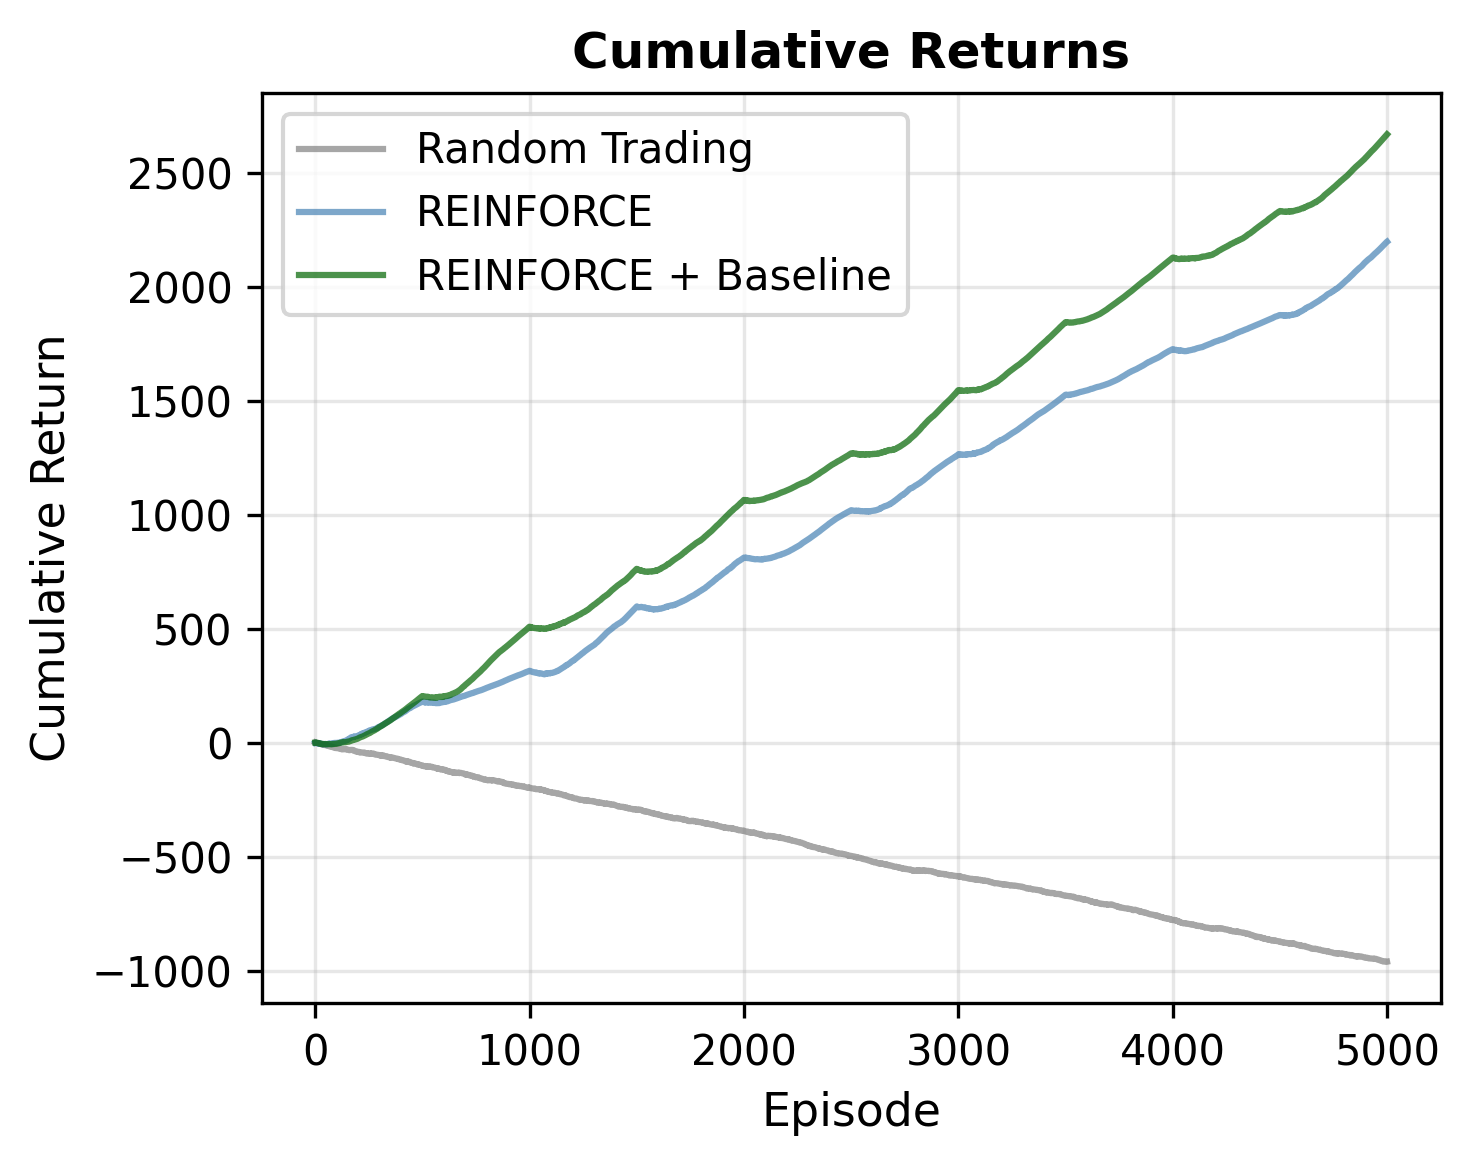
\includegraphics[width=\textwidth]{../report/figures/return_cumulative.png}
        \caption{Distribution of episode returns across 10 random seeds.}
        \label{fig:cumulative_return}
    \end{subfigure}
    \hfill
    \begin{subfigure}[t]{0.48\textwidth}
        \centering
        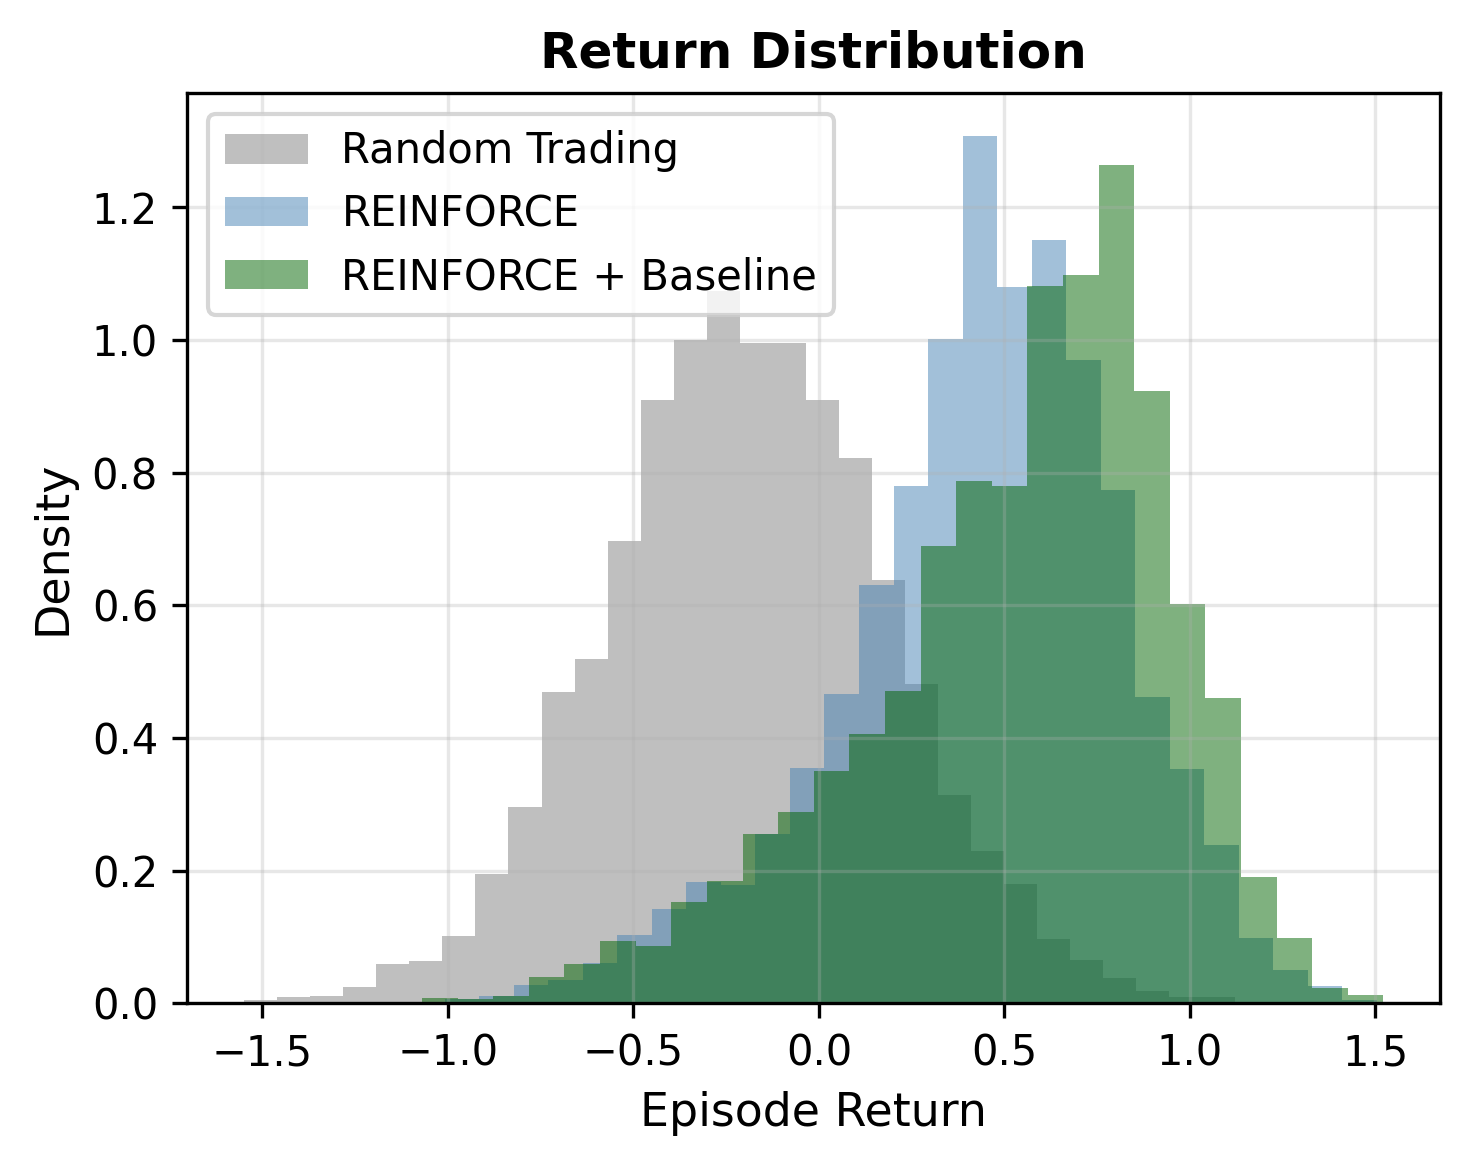
\includegraphics[width=\textwidth]{../report/figures/return_distribution.png}
        \caption{Cumulative portfolio return over the evaluation period.}
        \label{fig:return_distribution}
    \end{subfigure}
\end{figure}


Figure~\ref{fig:cumulative_return} presents cumulative portfolio performance. 
Both Monte Carlo agents achieve sustained positive growth, with the baseline variant showing 
a smoother trajectory and higher overall gains. In contrast, the random strategy demonstrates 
a steady downward trend, indicating no systematic profitability.

Figure~\ref{fig:return_distribution} shows the distribution of episode returns. 
REINFORCE with a baseline yields a tighter distribution concentrated around positive returns, 
indicating lower variance. The standard REINFORCE agent exhibits greater dispersion with occasional 
negative outcomes. The random policy is centered slightly below zero, reflecting the 
absence of learning and a tendency toward marginal losses.

\subsubsection{Summary of Quantitative Metrics}

\FloatBarrier % Prevent previous floats from interfering with table placement
\begin{table}[H]
\centering
\caption{Performance comparison across methods (averaged over 10 seeds).}
\label{tab:performance}
\resizebox{0.95\textwidth}{!}{%
\begin{tabular}{lcccccc}
\hline
Method & Mean Return & Std Dev & 95\% CI & SharpeRatio & Win Rate \\
\hline
REINFORCE+Baseline &  0.8177  &  0.1360 & [0.7204, 0.9149] & 20.5163 &  88.06  \\
REINFORCE & 0.6231 & 0.1745 & [0.4983, 0.7480] & 18.6067 & 87.94 \\
Random Policy &  -0.1925 & 0.0379 & [-0.2197, -0.1654] & -8.0677 & 30.48  \\

\hline
\end{tabular}%
}
\end{table}

Table~\ref{tab:performance} summarizes the key evaluation metrics, including mean final return, 
standard deviation, 95\% confidence interval, Sharpe ratio, and win rate (in percentage). 
The quantitative results confirm the visual evidence from the figures: 
REINFORCE with baseline consistently achieves higher returns, improved risk-adjusted performance, 
and reduced variability relative to standard REINFORCE. 
Both learning-based approaches substantially outperform the random trading strategy.

The confidence intervals show that both REINFORCE methods achieve positive returns, while the random policy does not. REINFORCE with a baseline has higher and more consistent returns, showing it learns a profitable and stable trading policy from historical data.

\FloatBarrier % Prevent figures from floating into the next section
